\documentclass{article}
\usepackage[utf8]{inputenc}

\usepackage[utf8]{inputenc}
\usepackage[spanish,es-tabla,es-nodecimaldot]{babel}
\usepackage{amsmath,amsthm,amsfonts,amssymb,mathtools,dsfont,mathrsfs}
\usepackage{enumerate,graphicx,xcolor}
\usepackage{lmodern}
\usepackage[T1]{fontenc}
\usepackage[left=2cm,top=2.5cm,right=2cm,bottom=2.5cm]{geometry}
\usepackage[activate={true,nocompatibility},final,tracking=true,kerning=true,spacing=true,factor=1100,stretch=10,shrink=10]{microtype}
\usepackage{hyperref}


%\DeclarePairedDelimiter{\norm}{\lVert}{\rVert}




\newcommand{\N}{\mathbb{N}}
\newcommand{\R}{\mathbb R}
\newcommand{\Z}{\mathbb Z}
\newcommand{\Rbar}{\overline{\mathbb R}}
\newcommand{\F}{\mathscr F}
\newcommand{\A}{\mathscr A}
\newcommand{\To}{\Rightarrow}
\newcommand{\C}{\mathscr C}
\newcommand{\La}{\mathscr L_A}
\newcommand{\B}{\mathcal B}
\newcommand{\Q}{\mathbb Q}
\renewcommand{\epsilon}{\varepsilon}
\renewcommand{\L}{\mathcal L}
\renewcommand{\d}{\mathrm d}
\newcommand{\abs}[1]{\left| #1 \right|}
\newcommand{\pts}[1]{\left( #1 \right)}
\newcommand{\norm}[1]{\left\lVert#1\right\rVert}
\renewcommand{\P}[1]{\mathbb P\left( #1 \right)}
\newcommand{\E}[1]{\mathbb E \left( #1 \right)}


\newcommand{\ols}[1]{\mskip.5\thinmuskip\overline{\mskip-.5\thinmuskip {#1} \mskip-.5\thinmuskip}\mskip.5\thinmuskip} % overline short
\newcommand{\olsi}[1]{\,\overline{\!{#1}}} % overline short italic
\makeatletter
\newcommand\closure[1]{
  \tctestifnum{\count@stringtoks{#1}>1} %checks if number of chars in arg > 1 (including '\')
  {\ols{#1}} %if arg is longer than just one char, e.g. \mathbb{Q}, \mathbb{F},...
  {\olsi{#1}} %if arg is just one char, e.g. K, L,...
}
% FROM TOKCYCLE:
\long\def\count@stringtoks#1{\tc@earg\count@toks{\string#1}}
\long\def\count@toks#1{\the\numexpr-1\count@@toks#1.\tc@endcnt}
\long\def\count@@toks#1#2\tc@endcnt{+1\tc@ifempty{#2}{\relax}{\count@@toks#2\tc@endcnt}}
\def\tc@ifempty#1{\tc@testxifx{\expandafter\relax\detokenize{#1}\relax}}
\long\def\tc@earg#1#2{\expandafter#1\expandafter{#2}}
\long\def\tctestifnum#1{\tctestifcon{\ifnum#1\relax}}
\long\def\tctestifcon#1{#1\expandafter\tc@exfirst\else\expandafter\tc@exsecond\fi}
\long\def\tc@testxifx{\tc@earg\tctestifx}
\long\def\tctestifx#1{\tctestifcon{\ifx#1}}
\long\def\tc@exfirst#1#2{#1}
\long\def\tc@exsecond#1#2{#2}
\makeatother

\newtheorem{lemma}{Lema}
\newtheorem{theorem}{Teorema}

\setlength\parindent{0pt}
\setlength\parskip{4pt}


\title{Cómputo científico para probabilidad y estadística. Tarea 8.\\
MCMC: MH con Kerneles Híbridos y Gibbs
Sampler}
\author{Juan Esaul González Rangel}
\date{Noviembre 2023}



\begin{document}

\maketitle


\begin{enumerate}

    \item Aplique el algoritmo de Metropolis-Hastings considerando como función 
    objetivo la distribución normal bivariada

    \[ f_{X_1,X_2}(\bar x) = \frac1{2\pi} |\Sigma|^{-1/2} \exp\left\{ -\frac12 
    (\bar x - \mu)'\Sigma^{-1}(\bar x - \mu) \right\} \]

    donde, 

    \[ \mu = \binom{\mu_1}{\mu_2} \quad \Sigma = \begin{pmatrix}
        \sigma_1^2 & \rho \sigma_1\sigma_2 \\
        \rho\sigma_1\sigma_2 & \sigma_2^2
    \end{pmatrix} \]
    
    Así, se tienen las siguientes distribuciones condicionales:
    
    \[ X_1 | X_2 = x_2 \sim N\left( \mu_1 + \rho \frac{\sigma_1}{\sigma_2}(x_2 - 
    \mu_2), \sigma_1^2(1 - \rho^2) \right) \]

    \[ X_2 | X_1 = x_1 \sim N\left( \mu_2 + \rho \frac{\sigma_2}{\sigma_1}(x_1 - 
    \mu_1), \sigma_2^2(1-\rho^2) \right) \]
    
    Considere las siguientes propuestas:

    \[ q_1 ((x_1',x_2') | (x_1,x_2)) = f_{X_1|X_2}(x_1'|x_2)\mathds 1_{(x_2' = x_2)}  \]

    \[ q_2 ((x_1',x_2') | (x_1,x_2)) = f_{X_2|X_1}(x_2'|x_1)\mathds 1_{(x_1' = x_1)}  \]

    
    A partir del algoritmo MH usando Kerneles híbridos simule valores de la distribución 
    normal bivariada, fijando $\sigma_1 = \sigma_2 = 1$, considere los casos 
    $\rho = 0.8$ y $\rho = 0.95$\footnote{Ver la tesis de Cricelio Montesinos para 
    una explicación más extensa del Gibbs, Montesinos, C (2016) ``Distribución de 
    Direcciones en el Gibbs Sampler Generalizad'', MSc Dissertation, CIMAT. 
    \url{https://www.cimat.mx/es/Tesis_digitales/}. También vean la Enciclopedia 
    de Estadística de Wiley, la entrada de \textit{Gibbs Sampler}: 
    \url{https://www.cimat.mx/~jac/2016WileytStatsRef_GibbsSampling.pdf.}}.


    \begin{proof}[Solución] Notemos que los kerneles de transición son la densidad de un 
        parámetro condicionada al valor que toman todos los otros parámetros, por lo que 
        el cociente de Metropolis-Hastings es exactamente 1 en ambos, y por lo tanto la 
        transición a la propuesta simepre se da.  Para evitar perder la aperiodicidad
        fuerte de la cadena, implementamos un tercer kernel de transición con una probabilidad
        muy baja que simplemente mantenga la posición actual. El kernel
        híbrido tiene la siguiente forma,

        \[ K = \sum_{i=1}^3 w_i K_i = 0.4999\left( f_{X_1|X_2}(x_1'|x_2)\mathds 1_{(x_2' = x_2)} 
        + f_{X_2|X_1}(x_2'|x_1)\mathds 1_{(x_1' = x_1)}\right) 
        + 0.0002(\mathds1_{(x_1'=x_1,x_2'=x_2)}).\]

        Al dejar fijo y tener aperiodicidad fuerte nos aseguramos de que la cadena es 
        ergódica y garantizamos la convergencia.

        Para la implementación de este algoritmo de MCMC, se definió la función 
        \texttt{mhbivar} que toma los siguientes parámetros;

        % mhbivar(iterations,mu=[0,0],rho=0.8,starting_point=np.array([0,0],dtype=float)):

        \begin{itemize}
            \item \texttt{iterations}: Cantidad de veces que se corre el algoritmo.
            \item \texttt{mu}: Vector de longitud 2 que representa la media de la 
            densidad objetivo, por defecto es \texttt{[0,0]}.
            \item \texttt{rho}: Coeficiente de correlación de las componentes, por 
            defecto es 0.8.
            \item \texttt{starting\_point}: Punto donde iniciar la cadena, por defecto 
            es \texttt{[0,0]}.
        \end{itemize}

        Se implementó el algoritmo para simular las siguientes densidades normales 
        multivariadas:

        \begin{center}
            \begin{tabular}{rllll}
                \hline
                \multicolumn{1}{l}{No.} & Media & Coeficiente de correlación & $\sigma_1$ & $\sigma_2$ \\ \hline
                1 & $(2,  3)$ & $\rho=0.8$  & 1 & 1 \\
                2 & $(-3, 2)$ & $\rho=0.95$ & 1 & 1 \\ \hline
                \end{tabular}
        \end{center}

        En la siguiente imagen se muestran las curvas de nivel de la primera densidad objetivo junto
        a 10,000 simulaciones realizadas con este kernel híbrido:

        \begin{center}
            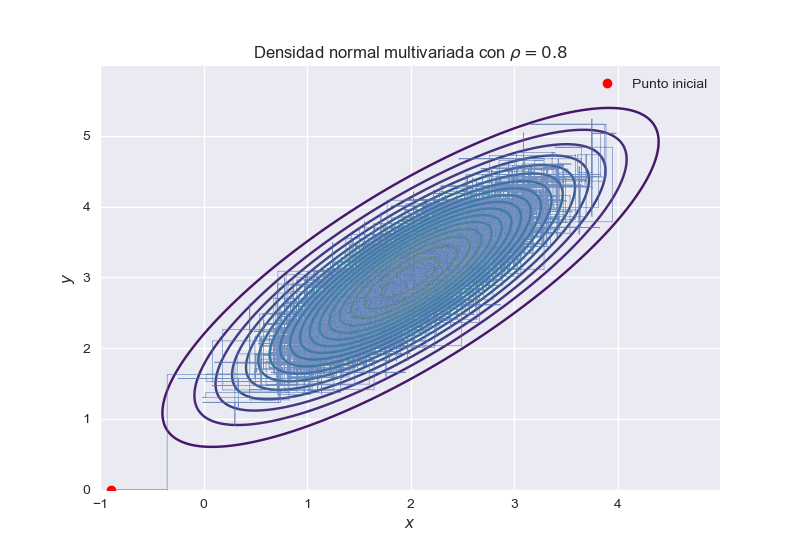
\includegraphics[width=0.75\textwidth]{Tarea8/traj11.png}
        \end{center}

        Podemos notar que el kernel sólo agrega nuevos puntos en las direcciones canónicas
        del plano, puesto que el muestreo de Gibbs estándar utiliza muestreo desde las 
        direcciones marginales. Además, a pesar de haber comenzado en un punto alejado de 
        la media, el algoritmo converge rápidamente y tenemos un muestreo efectivo desde las
        regiones con más masa de la distribución. 
        
        Para mejorar el muestreo, podemos retirar
        las primeras iteraciones de la cadena, y para esto usamos la siguiente gráfica de 
        burn-in en la que comparamos el logaritmo de la densidad evaluada en $X_t$
        con las iteraciones de la cadena. 

        \begin{center}
            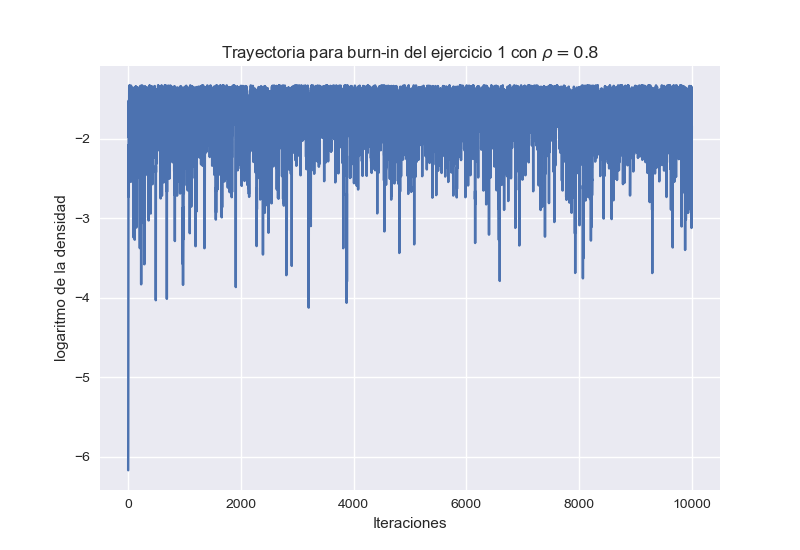
\includegraphics[width=0.75\textwidth]{Tarea8/burnin1.png}
        \end{center}

        En la gráfica notamos que en pocas iteraciones se estabiliza el 
        logaritmo de la densidad evaluada en la cadena, por lo que la cadena parece 
        converger de manera rápida. Basta eliminar los primeros 100 puntos para 
        tener un comportamiento uniforme.

        Para la segunda normal, tenemos la siguiente gráfica de su muestreo,

        \begin{center}
            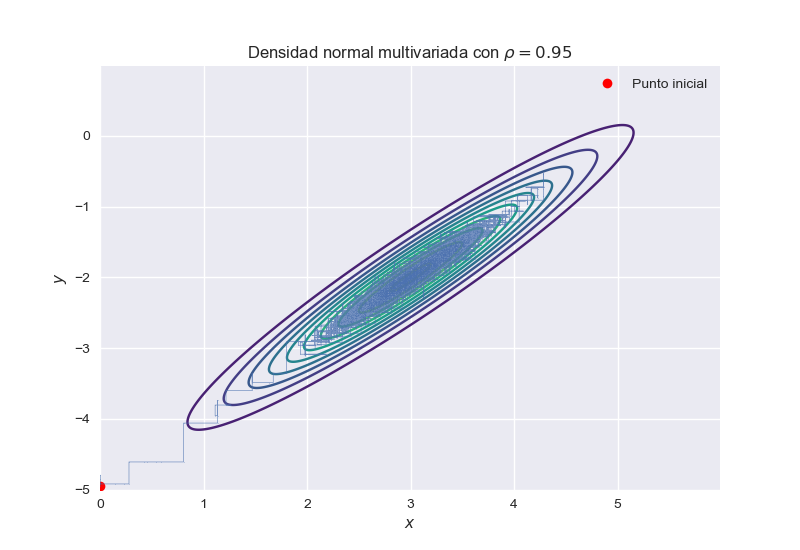
\includegraphics[width=0.75\textwidth]{Tarea8/traj12.png}
        \end{center}

        Al igual que en el caso anterior, observamos que punto inicial se encuentra
        relativamente alejado de la media de la dsitribución, pero al avanzar nos acercamos a
        muestrear más rápidamente de los puntos donde la distribución acumula más masa.

        La gráfica de burn-in para este muestreo es la siguiente;

        \begin{center}
            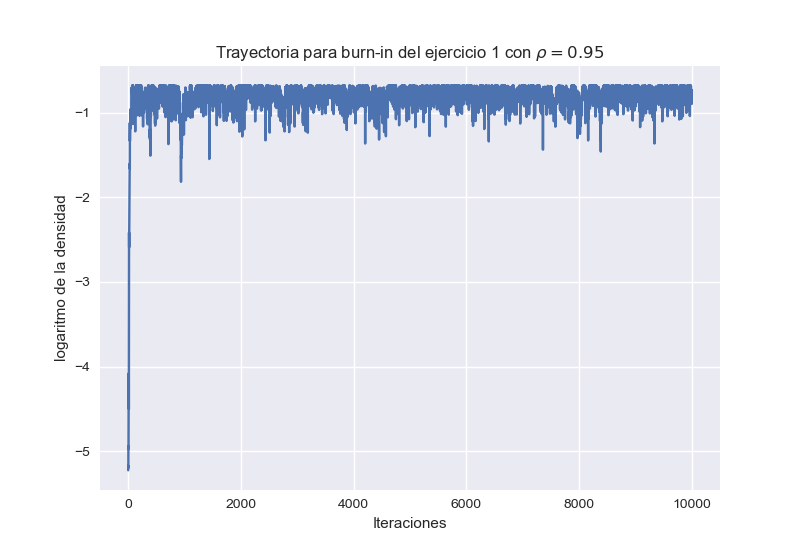
\includegraphics[width=0.7\textwidth]{Tarea8/burnin2.png}
        \end{center}

        Se tiene un comportamiento menos uniforme que en el primer muestreo, y esto lo notamos
        en el hecho de que hay más diferencia entre los primeros valores del logaritmo
        de la densidad, pero en pocas iteraciones el comportamiento se estabiliza. En este
        caso también basta eliminar los primeros 100 puntos para tener un comportamiento
        uniforme y por lo tanto un muestreo más adecuado de la distribución.

        Como estamos muestreando de una distribución conocida, es sencillo encontrar
        las marginales de nuestra normal multivariada. En la siguiente figura se 
        incluyen los histogramas de las marginales de cada una de las normales 
        bivariadas muestreadas y se comparan con la densidad real.

        \begin{center}
            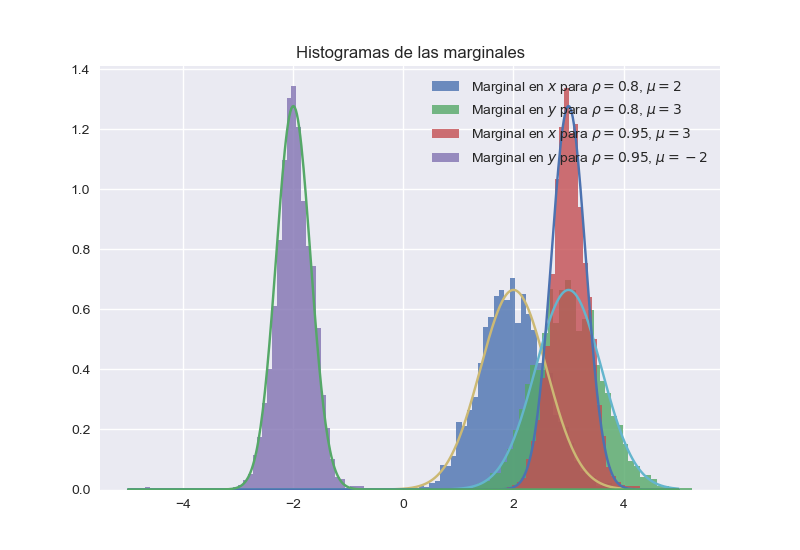
\includegraphics[width=0.75\textwidth]{Tarea8/hist_dens.png}
        \end{center}

        En las gráfinas notamos que el ajuste de los histogramas a la densidad real 
        es bastante bueno.


    \end{proof}



    \item Considere los tiempos de falla $t_1, \dots, t_n$ con distribución 
    \textit{Weibull}$(\alpha, \lambda)$:
    
    \[ f (t_i|\alpha, \lambda) = \alpha\lambda t^{\alpha-1}_i e^{-t^\alpha_i 
    \lambda} \]
    
    Se asumen como a priori $\alpha \sim \exp(c)$ y $\lambda|\alpha \sim 
    $Gama$(\alpha, b)$, por lo tanto, $f (\alpha, \lambda) = f (\lambda|\alpha) 
    f (\alpha)$\footnote{Este ejemplo aparece en Kundu, D. (2008), ``Bayesian 
    Inference and Life Testing Plan for the Weibull Distribution in Presence of 
    Progressive Censoring'', Technometrics, 50(2), 144–154.}. Así, para la 
    distribución posterior se tiene:
    
    \[f (\alpha, \lambda|\bar t) \propto f (\bar t|\alpha, \lambda)f (\alpha, 
    \lambda)\]
    
    A partir del algoritmo MH usando Kerneles híbridos simule valores de la distribución 
    posterior $f(\alpha, \lambda|\bar t)$, considerando las siguientes propuestas:


    \underline{Propuesta 1}:

    \[ \lambda_p|\alpha, \bar t \sim Gama \left(\alpha + n , b +\sum_{i=1}^n 
    t^\alpha_i \right) \quad \text{y dejando $\alpha$ fijo.} \]

    \underline{Propuesta 2:}

    \[\alpha_p|\lambda, \bar t \sim Gama (n + 1 , -\log(b) - \log(r_1) + c), 
    \text{ con } r_1 = \prod_{i=1}^n t_i \text{ y dejando $\lambda$ fijo. }\]
    
    \underline{Propuesta 3:}
    
    $\alpha_p \sim \exp(c)$ y $\lambda_p|\alpha_p \sim Gama(\alpha_p, b)$.

    \underline{Propuesta 4 (RWMH):} 
    
    $\alpha_p = \alpha + \epsilon$, con $\epsilon \sim N (0, \sigma)$ y dejando 
    $\lambda$ fijo. 
    
    Simular datos usando $\alpha = 1$ y $\lambda = 1$ con $n = 20$. 
    Para la a priori usar $c = 1$ y $b = 1$.

    \begin{proof}[Solución]
        Para la implementación de este algoritmo MCMC es necesario notar ciertos
        aspectos de cada una de las propuestas que pueden simplificar los cálculos
        o resultar problemáticos. Para la propuesta 1, vemos que se trata de un 
        kernel de Gibbs al estar muestreando desde la condicional de un parámetro
        dados todos los demás, esto hace que sepamos de antemano que el cociente de
        Metropolis-Hastings para esta propuesta es 1, y por lo tanto siempre se acepta
        la transición. 
        
        Para la propuesta 2, el término $-\log(b)-\log(r_1)+c$ puede 
        ser negativo dependiendo de $r_1$, y por lo tanto podría darse el caso de que
        se estuviera tratando de simular desde una distribución gamma con parámetro
        negativo, lo cuál no tiene sentido. Para evitar este problema, incluimos un
        condicional, de manera que si el término resulta negativo, no se proponga la 
        transición y de esta manera el segundo kernel nos sirva como una manera de
        asegurar la aperiodicidad fuerte de la cadena. 

        En la cuarta propuesta tenemos que la transición es simétrica, pues se trata de
        un RWMH, con lo que es necesario únicamente comparar las densidades objetivo 
        $f(y)$ y $f(x)$ para evaluar si se acepta o rechaza la propuesta.

        Al considerar estos aspectos, se implementó la función \texttt{MHposter} que 
        recibe argumentos como el número de iteraciones, el punto inicial y los 
        parámetros de las distribuciones a usar. 

        La siguiente imagen muestra la trayectoria de 10,000 simulaciones de la objetivo usando este
        kernel híbrido con igual peso a cada propuesta,

        \begin{center}
            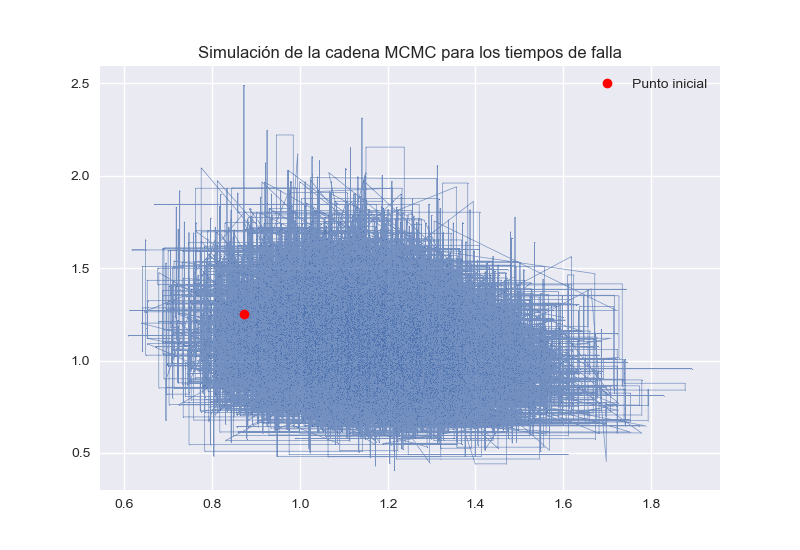
\includegraphics[width=0.8\textwidth]{Tarea8/traj2.png}
        \end{center}

        Algo que podemos notar es que la mayor cantidad de líneas que se ven están en
        dirección horizontal o vertical, lo que significa que la mayor parte de las
        transiciones vienen de las propuestas que mueven únicamente al parámetro 
        $\alpha$ o al $\lambda$ cada vez.

        Los histogramas de las marginales de $\alpha$ y $\lambda$ se obervan en las
        siguientes figuras.

        \begin{center}
            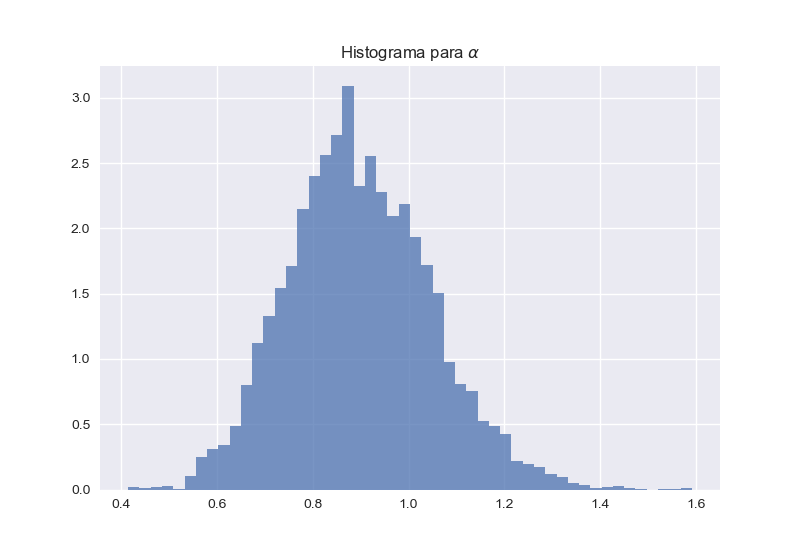
\includegraphics[width=0.7\textwidth]{Tarea8/hist21.png}
        \end{center}

        \begin{center}
            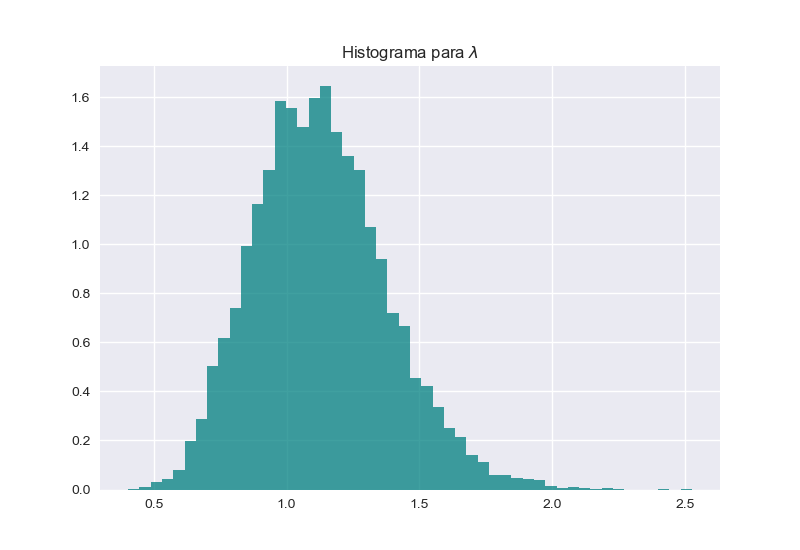
\includegraphics[width=0.7\textwidth]{Tarea8/hist22.png}
        \end{center}

        Como sabemos que los datos con los que formamos la posterior vienen de una 
        distribución Weibull$(1,1)$, es de interés conocer cuál sería el estimador
        de los parámetros si usamos este muestreo de MCMC. El estimador más sencillo
        de usar es la media de los datos simulados, que por la Ley de Grandes Números
        aproxima al estimador de Bayes. El vector de medias de este muestreo es 
        $(1.1536,1.1136)$, que aproxima bien al original $(1,1)$, considerando que 
        sólo se tienen 20 observaciones de los datos.


        En esta cadena también es útil conocer el burn-in para saber cuántos datos 
        iniciales deberíamos descartar para asegurar que muestreamos desde la objetivo.
        La gráfica de iteraciones contra $\log(f(X_t))$  se muestra a 
        continuación.

        \begin{center}
            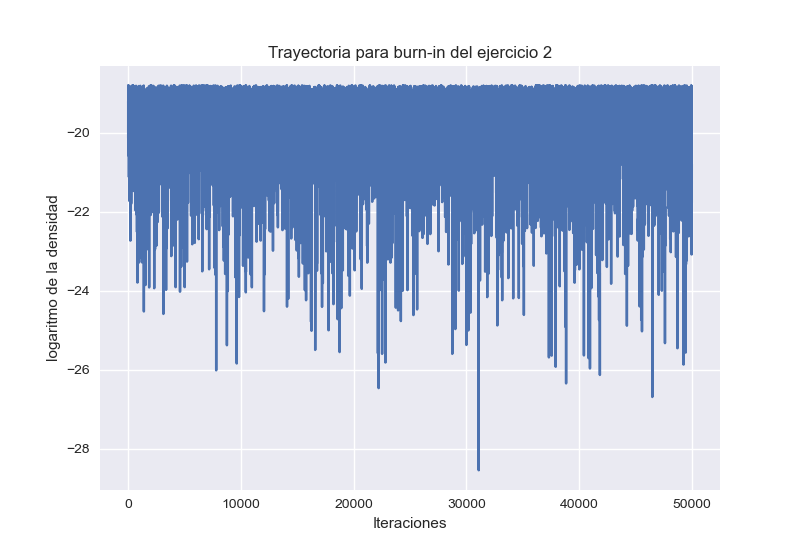
\includegraphics[width=0.7\textwidth]{Tarea8/burnin3.png}
        \end{center}

        El comprtamiento del logaritmo de la densidad es bastante uniforme, por lo que 
        podemos considerar que la cadena muestrea de la dsitribución desde el principio.\end{proof}

    \item Considere el ejemplo referente al número de fallas de bombas de agua en 
    una central nuclear\footnote{Este ejemplo fue usado en el artículo original 
    del Gibbs sampler del Gelfand y Smith (1990). Vea también Norton, R.A., 
    Christen, J.A. y Fox, C. (2017), ``Sampling hyperparameters in hierarchical 
    models: improving on Gibbs for high-dimensional latent fields and large data 
    set'' Communications in Statistics - Simulation and Computation, 
    \url{http://dx.doi.org/10.1080/03610918.2017.1353618}}, donde $p_i$ 
    representa el número de fallas en el tiempo de operación $t_i$, con $i = 1, 
    \dots, n$.

    Se considera el modelo $p_i \sim $Poisson$(\lambda_i t_i)$, (las $\lambda_i$ 
    son independientes entre si), con distribuciones a priori $\lambda_i|\beta 
    \sim Gama(\alpha, \beta)$ y $\beta \sim Gama(\gamma, \delta)$, por lo tanto:
    
    \[f (\lambda_1, \dots , \lambda_n, \beta) = f (\lambda_1|\beta)f (\lambda_2|
    \beta) \dots f(\lambda_n|\beta)f(\beta)\]
    
    Para la distribución posterior se tiene:
    
    \[f (\lambda_1, \dots , \lambda_n, \beta|\bar p) \propto L(\bar p, \bar \lambda,
     \beta)f (\lambda_1, \dots , \lambda_n, \beta)\]
    
    Simule valores de la distribución posterior $f (\lambda_1, \dots , \lambda_n, 
    \beta|\bar p)$, usando un kernel híbrido, considerando las propuestas: 
    
    \[\lambda_i|\bar \lambda_{-i}, \beta, \bar t \sim Gama(p_i + \alpha , \beta + 
    t_i)\]

    \begin{table}[!h] \centering
        \begin{tabular}{|l|l|l|l|l|l|l|l|l|l|l|}
            \hline
            Bomba ($i$)         & 1     & 2     & 3     & 4      & 5    & 6     & 7    & 8    & 9   & 10    \\ \hline
            T. de uso ($t_i$)    & 94.32 & 15.72 & 62.88 & 125.76 & 5.24 & 31.44 & 1.05 & 1.05 & 2.1 & 10.48 \\ \hline
            \# de fallas ($p_i$) & 5     & 1     & 5     & 14     & 3    & 17    & 1    & 1    & 4   & 22    \\ \hline
        \end{tabular} 
        \label{tab1}
        \caption{Datos de bombas de agua en centrales nucleares (Robert y Casella,
        p. 385) para el ejemplo 8.3.}
    \end{table}



    \[\beta|\bar \lambda, \bar t \sim Gama \left( n\alpha + \gamma , \delta + 
    \sum_{i=1}^n\lambda_i \right).\]
    
    Verifique que estas son propuestas Gibbs.

    Use los datos del Cuadro 1 con los parámetros a priori $\alpha = 1.8, 
    \gamma = 0.01$ y $\delta = 1$.

    \begin{proof}[Solución] 
        Mostramos primero que las propuestas dadas son de Gibbs. La verosimilitud es,

        \begin{align*}
            L(\bar p, \bar\lambda, \beta) &= \prod_{i=1}^n \frac{ (\lambda_i 
            t_i)^{p_i} e^{-\lambda_i t_i} }{(p_i)!}.
        \end{align*}

        La posterior conjunta se obtiene multiplicando la verosimilitud anterior por las
        dsitribuciones a priori,

        \begin{align*}
        L(\bar p, \bar\lambda, \beta)f(\lambda_1,\dots,\lambda_n,\beta) 
        &= L(\bar p,\bar\lambda,\beta)f(\lambda_1|\beta)f(\lambda_2|\beta)\dots f(\lambda_n|\beta)f(\beta),\\
        &= \prod_{i=1}^n \left\{ \frac{ (\lambda_i t_i)^{p_i} e^{-\lambda_i t_i} }{(p_i)!}\right\}
        \frac{\beta e^{-\beta\lambda_1}(\beta\lambda_1)^{\alpha-1}}{\Gamma(\alpha)} \cdots
        \frac{\beta e^{-\beta\lambda_n}(\beta\lambda_n)^{\alpha-1}}{\Gamma(\alpha)}
        \frac{\delta e^{-\delta\beta}(\delta\beta)^{\gamma-1}}{\Gamma(\gamma)}
        \end{align*}.
    \end{proof}

    Para encontrar $f_{\lambda_i|\bar\lambda_{-i},\beta,\bar t}$, tomamos en la expresión
    anterior únicamente los términos que dependen de $\lambda_i$ para un $i$ específico.

    \begin{align*}
        f_{\lambda_i|\bar\lambda_{-i},\beta,\bar t} 
        &\propto \left(\frac{(\lambda_i t_i)^{p_i}e^{-\lambda_i t_i}}{p_i!}\right)
        \left( \frac{\beta e^{-\beta\lambda_i}(\beta\lambda_i)^{\alpha-1}}{\Gamma(\alpha)} \right)
        \propto \lambda_i^{p_i+\alpha-1}e^{-(\beta+t_i)\lambda_i}
    \end{align*}

    La expresión resultante es el núcleo de una densidad Gamma con parámetros $p_i+\alpha$ 
    y $\beta+t_i$, por lo que conluimos que al agregar las constantes de normalización,
    tenemos que $\lambda_i|\bar\lambda_{-i},\beta,\bar t\sim Gamma(p_i+\alpha,\beta+t_i)$.

    De manera completamente análoga, encontramos $f_{\beta|\bar\lambda,\bar t}$,

    \begin{align*}
        f_{\beta|\bar\lambda,\bar t} 
        &\propto \prod_{i=1}^n \left\{ \frac{ (\lambda_i t_i)^{p_i} e^{-\lambda_i t_i} }{(p_i)!}\right\}
        \frac{\beta e^{-\beta\lambda_1}(\beta\lambda_1)^{\alpha-1}}{\Gamma(\alpha)} \cdots
        \frac{\beta e^{-\beta\lambda_n}(\beta\lambda_n)^{\alpha-1}}{\Gamma(\alpha)}
        \frac{\delta e^{-\delta\beta}(\delta\beta)^{\gamma-1}}{\Gamma(\gamma)},\\
        &\propto e^{-\left(\sum_{i=1}^n\lambda_i -\delta\right)\beta} \beta^{n\alpha+\gamma-1}.
    \end{align*}

    De nuevo, la expresión al final es el núcleo de una densidad $Gamma\left(n\alpha+\gamma
    , \delta + \sum_{i=1}^n \lambda_i \right)$, por lo que concluimos que al agregar las
    constantes de normalización, esta es la dsitrbiución posterior de $\beta$ dados los
    datos y los parámetros $\lambda_i$. Entonces las propuestas dadas son de Gibbs y por
    lo tanto sabemos que la probabilidad de aceptación de la propuesta es 1.

    El que los núcleos de transición sean Gibbs nos da la ventaja de que no es necesario 
    caalcular el cociente de Metropolis-Hastings, pero introduce el problema de que es
    probable perder la aperiodicidad fuerte del proceso. Para recuperar esta propiedad
    y garantizar que la cadena sea ergódica, introducimos en el código una probabilidad
    de 0.0001 de que no se elija ningún kernel de transición, y en su lugar se permanezca
    en el mismo punto.

    En la función \texttt{MHpump} del archivo \texttt{Tarea8.py} se implementa este 
    algoritmo y toma como arguentos \texttt{iterations} que es la cantidad de veces
    que se repite el algoritmo y \texttt{starting\_point} que es el punto inicial de
    la cadena. 
    
    Al realizar 50,000 iteraciones usando el punto inicial $(1,1,1,1,1,1,1,1,1,1,1)$
    encontramos los siguientes histogramas para cada uno de los parámetros,

    \begin{center}
        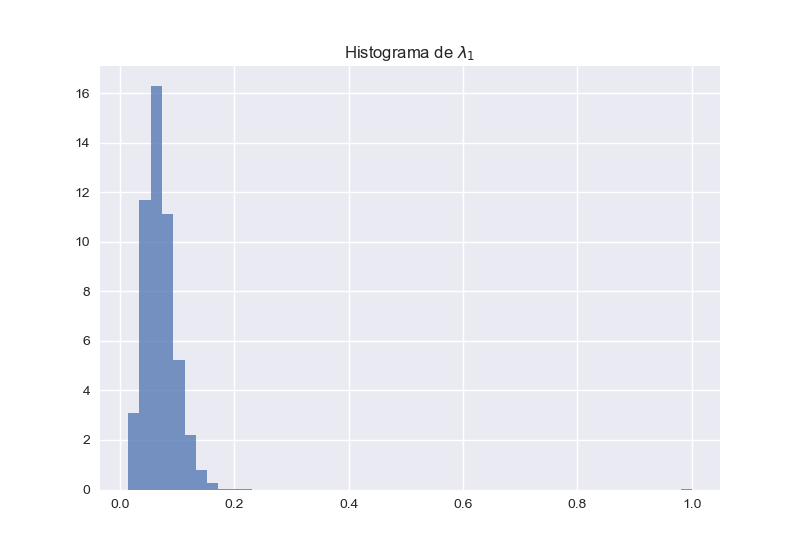
\includegraphics[width=0.8\textwidth]{Tarea8/hist0.png}
        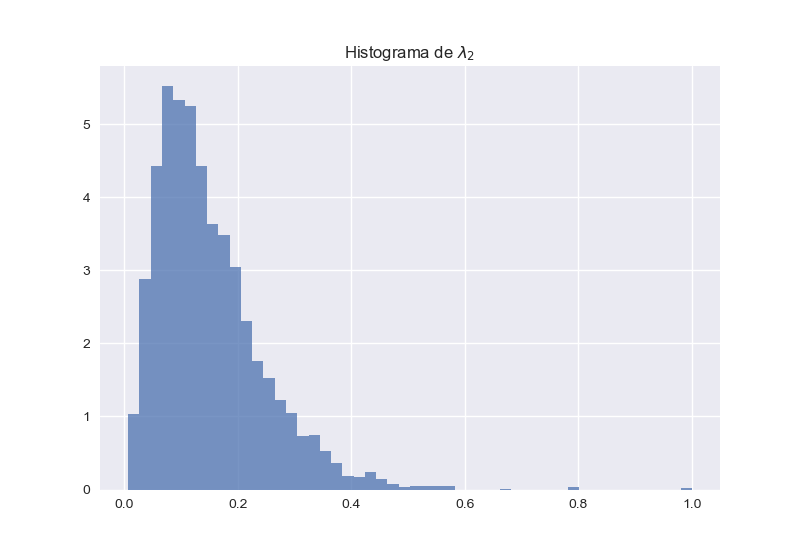
\includegraphics[width=0.8\textwidth]{Tarea8/hist1.png}
        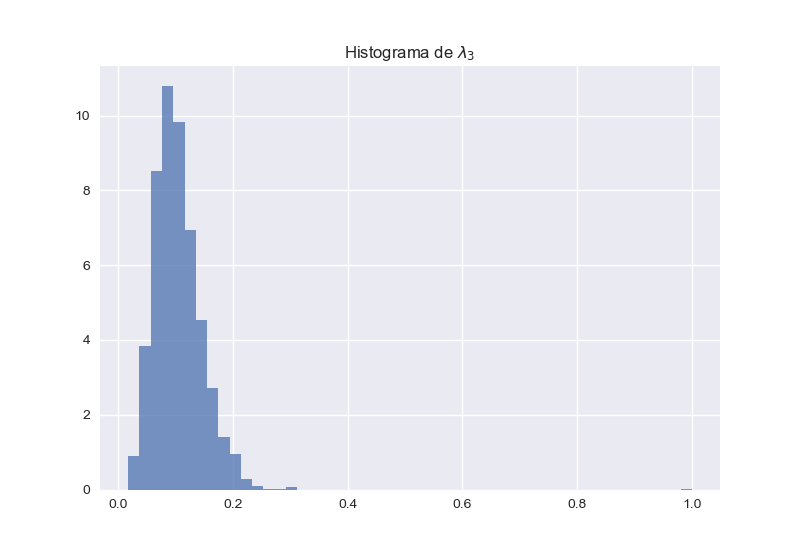
\includegraphics[width=0.8\textwidth]{Tarea8/hist2.png}
        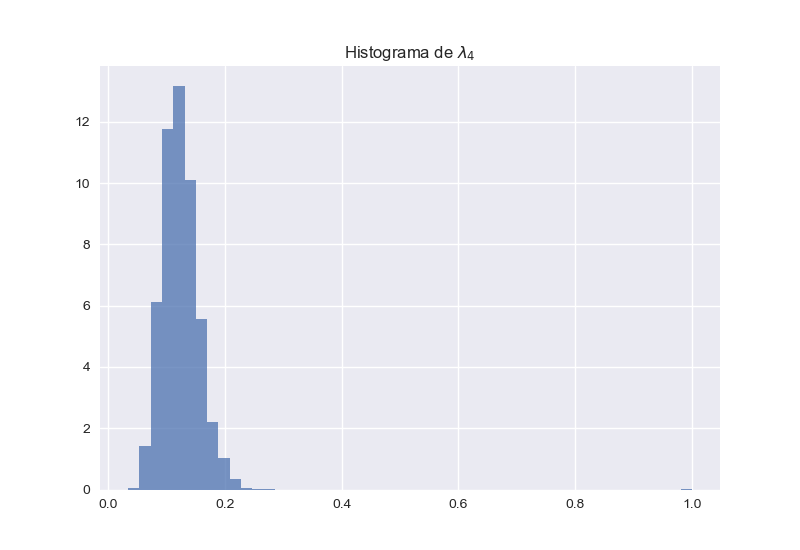
\includegraphics[width=0.8\textwidth]{Tarea8/hist3.png}
        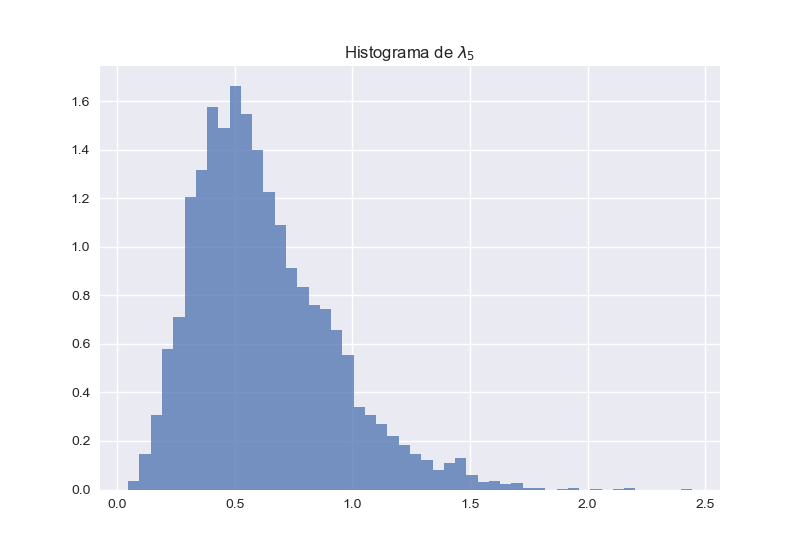
\includegraphics[width=0.8\textwidth]{Tarea8/hist4.png}
        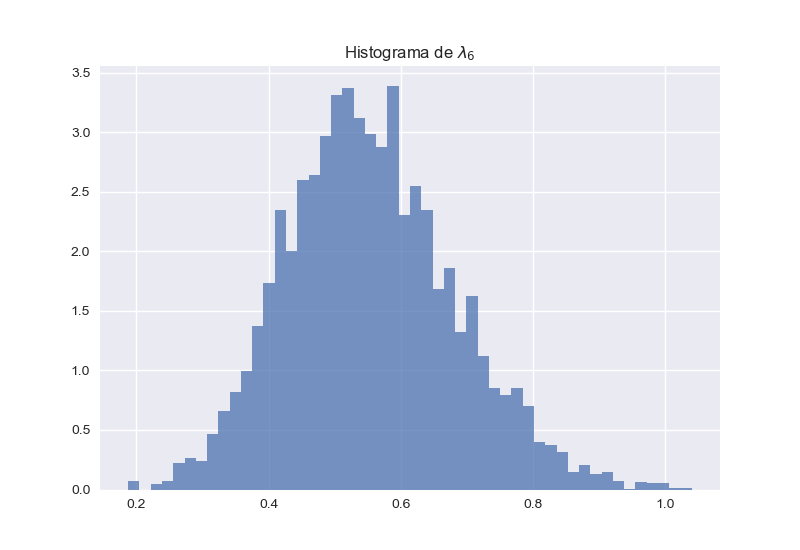
\includegraphics[width=0.8\textwidth]{Tarea8/hist5.png}
        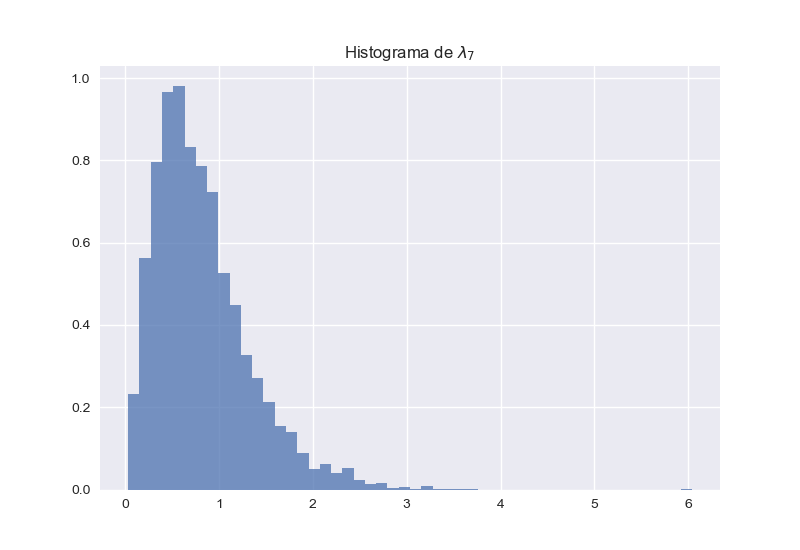
\includegraphics[width=0.8\textwidth]{Tarea8/hist6.png}
        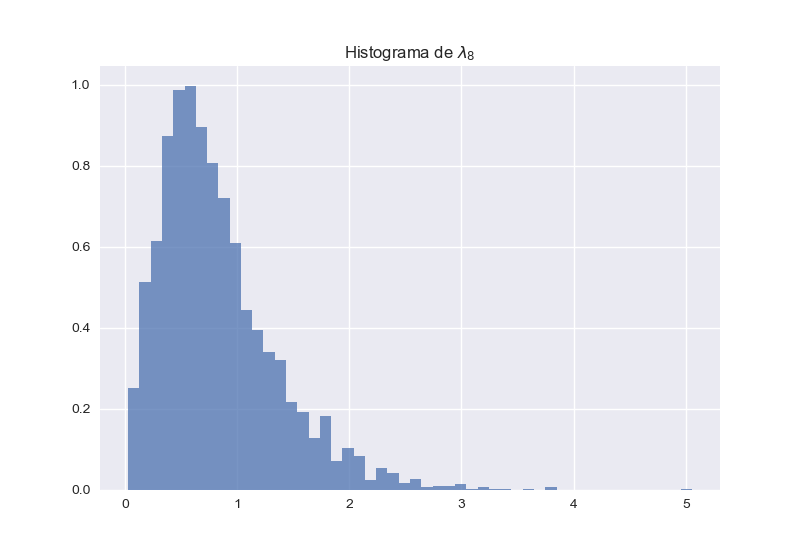
\includegraphics[width=0.8\textwidth]{Tarea8/hist7.png}
        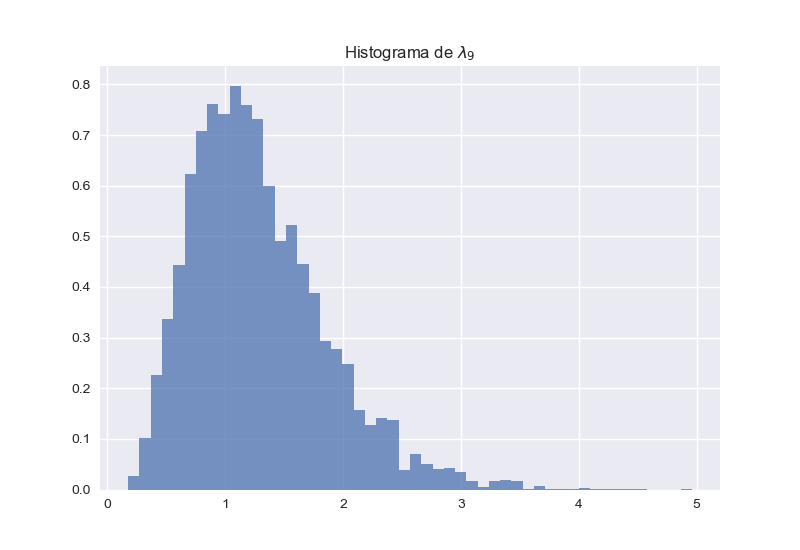
\includegraphics[width=0.8\textwidth]{Tarea8/hist8.png}
        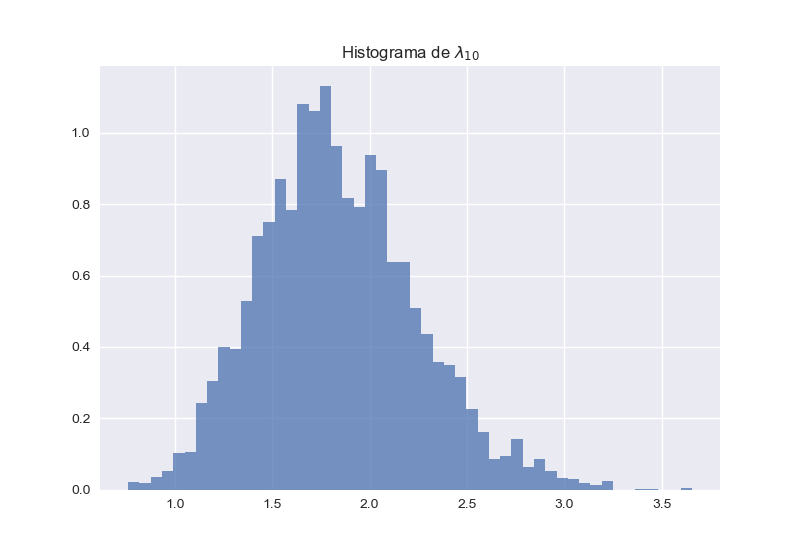
\includegraphics[width=0.8\textwidth]{Tarea8/hist9.png}
        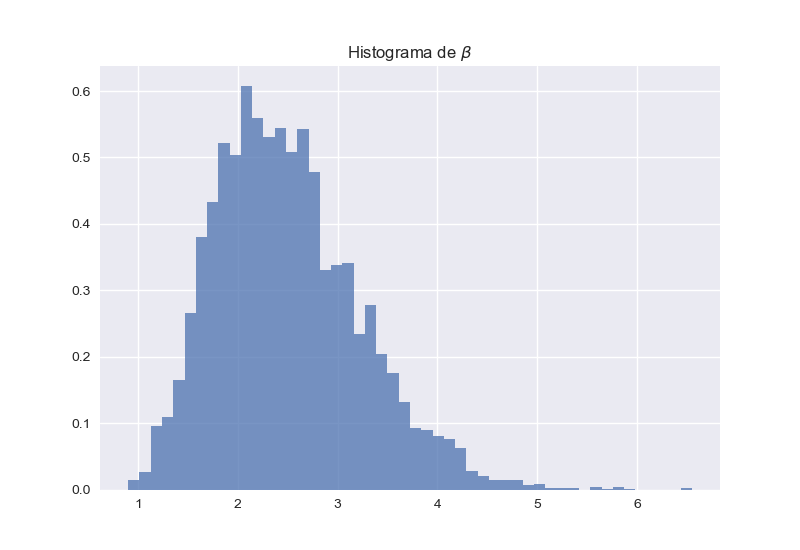
\includegraphics[width=0.8\textwidth]{Tarea8/hist10.png}
    \end{center}

    Como se trata de una distribución en 11 dimensiones, no es posible representar la
    transición de la cadena en una imagen bidimensional, pero podemos usar los datos 
    con los que contamos para encontrar estimadores de $\lambda_i$ y $\beta$. Al tomar
    la media de los datos muestreados tenemos los siguientes estimadores;

    \begin{itemize}
        \item $\lambda_1 = 0.07022$.
        \item $\lambda_2 = 0.1497$.
        \item $\lambda_3 = 0.1038$.
        \item $\lambda_4 = 0.1232$.
        \item $\lambda_5 = 0.6243$.
        \item $\lambda_6 = 0.5545$.
        \item $\lambda_7 = 0.8221$.
        \item $\lambda_8 = 0.8243$.
        \item $\lambda_9 = 1.2836$.
        \item $\lambda_{10} = 1.8418$.
        \item $\beta = 2.4976$.
    \end{itemize}





   
\end{enumerate}




 \end{document}